\documentclass{article}

\usepackage[T1]{fontenc}
\usepackage{graphicx}
\usepackage{fancyhdr}
\pagestyle{fancy}
\fancyhf{}
\lhead{Draft 0.1}
\rhead{Elliot Oram}
\rfoot{\thepage}


\title{Charades Class Diagram}
\author{elo9@aber.ac.uk}

\begin{document}

\maketitle
\tableofcontents

\newpage

\section{Charades Class Diagram}
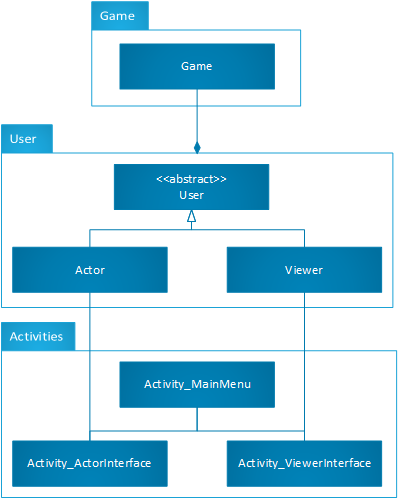
\includegraphics[width=\textwidth]{CharadesClassImage}

\newpage


\section{Description of Class Diagram}
\subsection{Game}

\subsection{User}

\subsection{Activities}
Activities are the andriod equivalent of graphical users interfaces. Each activity corresponds to a different screen on the app.
The main menu activity will show the splash screen for the Charades Game.
The Actor interface will only be shown to the actor in the the Staging Area and will allow the Actor to choose the phrase and current word to act out. The Actor will also be informed if the word or phrase they are acting has been guessed correctly.
The Viewer interface will display the current word in the phrase that is viewer are attempting to guess, as well as the genre of the phrase (e.g. book, film, television show, ect.). This interface will give the option to guess either the word or the whole phrase and a submit button to submit a guess. The interface will inform the viewer if the guess is correct or not.


\end{document}